\documentclass[12pt,a4paper,oneside]{memoir}
\usepackage[top=1cm,left=1cm,right=1.5cm,bottom=2cm]{geometry}
\usepackage[spanish]{babel}
\usepackage[utf8]{inputenc}
\usepackage{csquotes}
\usepackage[colorlinks=true,urlcolor=magenta,citecolor=red,linkcolor=violet,bookmarks=true]{hyperref}
\usepackage[style=apa,citestyle=numeric,sorting=nyt,sortcites=true,autopunct=true,autolang=hyphen,hyperref=true,abbreviate=false,backref=true,backend=biber,defernumbers=true]{biblatex}
\usepackage[many]{tcolorbox}
\usepackage[T1]{fontenc}
\usepackage{makeidx}
\usepackage{lscape}
\usepackage{pdflscape}
\usepackage{epstopdf}
\usepackage{booktabs}
\usepackage{pdfpages}
\usepackage{textcomp}
\usepackage{empheq}
\usepackage{tasks}
\usepackage{array}
\usepackage{tikz}
\usepackage{lipsum}
\usepackage{indentfirst}
\usepackage{graphicx}
\usepackage{subfig}
\usepackage{float}
\usepackage{blindtext}
\usepackage{tabularx}
\usepackage{ragged2e}
\usepackage{xcolor}
\usepackage{multirow}
\usepackage{bookmark}
\usepackage{amsmath,amssymb,amsthm}
\usepackage{lastpage}
\usepackage{epigraph}
\usepackage{enumerate}
\usepackage{enumitem}

\newlist{questions}{enumerate}{3}
\setlist[questions]{label=\arabic*.}
\newcommand{\question}{\item}
\setlist[enumerate,1]{(leftmargin=*, itemsep=12pt, label={\textbf{\arabic*.)}}}

\newlist{partes}{enumerate}{3}
\setlist[partes]{label=(\alph*)}
\newcommand{\parte}{\item}
%---
\newlist{subpartes}{enumerate}{3}
\setlist[subpartes]{label=\roman*)}
\newcommand{\subparte}{\item}

\newcommand*\circled[1]{\tikz[baseline=(char.base)]{\node[shape=circle,draw,inner sep=2pt] (char) {#1};}}

\pagestyle{plain}
\newcommand{\instituto}{Universidad Sergio Arboleda}
\newcommand{\curso}{Algebra Lineal 1}
\newcommand{\professor}{Alejandro Garzón}
\newcommand{\disciplina}{Matemáticas}
\newcommand{\titulo}{Taller}
\newcommand{\alumnoI}{Juan Sebastián Caballero Bernal}
\newcommand{\alumnoII}{Luz Angela Orjuela Nieto}
\linespread{1.5}

\newtheorem*{definition*}{Definición}
\newtheorem*{theorem*}{Teorema}
\newtheorem*{axiom*}{Postulado}
\newtheorem{theorem}{Teorema}[section]
\renewcommand*{\proofname}{\textbf{Demostración:}}

%\addbibresource{bibliography.bib}
%\defbibheading{bibempty}{}

%%%%%%%%%%%%%%%%%%%%%%%%%%%%%%%%%%%%%%%%%%%%%%%%%%%%%%%%
%                      Encabezado                      %
%%%%%%%%%%%%%%%%%%%%%%%%%%%%%%%%%%%%%%%%%%%%%%%%%%%%%%%%
\begin{document}
\begin{table}[H]
\centering
\begin{tabular*}{\textwidth}{l@{\extracolsep{\fill}}l@{\extracolsep{\fill}}}
    \begin{tabular}[l]{@{}l@{}}
        \textbf{\instituto}\\
        \textbf{Disciplina: \disciplina}\\
        \textbf{Profesor: \professor}\\ 
    \end{tabular} & 
    \begin{tabular}[l]{@{}l@{}}
        {\curso}\\
        {\alumnoI}\\
        {\alumnoII}\\
    \end{tabular}
\end{tabular*}
\end{table}
\begin{center}
\rule[2ex]{\textwidth}{1pt}
{\Large{\titulo}}
\end{center}
\rule[2ex]{\textwidth}{1pt}

%%%%%%%%%%%%%%%%%%%%%%%%%%%%%%%%%%%%%%%%%%%%%%%%%%%%%%%%
%                       Preguntas                      %
%%%%%%%%%%%%%%%%%%%%%%%%%%%%%%%%%%%%%%%%%%%%%%%%%%%%%%%%

\begin{questions}[label=\protect\circled{\bfseries\arabic*}]
\question \textbf{Pregunta 36:} Determinar si la siguiente afirmación es verdadera o falsa:

\begin{quote}
    Si $v_1, \dots, v_4$ son vectores en $\mathbb{R}^4$ y $v_3$ no es una combinación lineal de $v_1, v_2, v_4$. Entonces $\{v_1, v_2, v_3, v_4\}$ es linearmente independiente.
\end{quote}

Eso es falso. Como contraejemplo, tome:
$$\begin{matrix}
    v_1 = \begin{bmatrix}
        0 \\ 0 \\ 0 \\ 0
    \end{bmatrix} & v_2 = \begin{bmatrix}
        0 \\ 1 \\ 0 \\ 0
    \end{bmatrix} & v_3 = \begin{bmatrix}
        0 \\ 0 \\ 1 \\ 4
    \end{bmatrix} & v_4 = \begin{bmatrix}
        0 \\ 0 \\ 1 \\ 0
    \end{bmatrix}
\end{matrix}$$
Es fácil comprobar que $v_3$ no es una combinación lineal de los otros tres vectores, pues al hacer la matriz
aumentada correspondiente a la ecuación matricial $x_1v_1 + x_2v_2 + x_3v_4 = v_3$ se tendrá:
\begin{align*}
    \begin{pmatrix}
        0 & 0 & 0 & 0\\
        0 & 1 & 0 & 0\\
        0 & 0 & 1 & 1\\
        0 & 0 & 0 & 4
    \end{pmatrix}
\end{align*} 
Es evidente que la matriz representa un sistema inconsistente. Por tanto, $v_3$ no es una combinación lineal de los otros vectores. Pero por
el \textit{Teorema 9} se puede deducir que el sistema es linealmente dependiente puesto que $v_1$ es el vector cero.

\question \textbf{Pregunta 36:} Sea $T : \mathbb{R}^3 \to \mathbb{R}^3$ la transformación lineal que proyecta cada vector $x = (x_1, x_2, x_3)$ el plano
$x_2 = 0$, de forma que $T(x) = (x_1, 0, x_3)$. Demostrar que $T$ es una transformación lineal.
\begin{proof}
    Para empezar, demostraremos que la suma de vectores se mantiene por la función. Esto será que para $x = (x_1, x_2, x_3)$ y $y = (y_1, y_2, y_3)$ tendremos:
    \begin{align*}
        T(x + y) &= T((x_1, x_2, x_3) + (y_1, y_2, y_3))\\
        &= T((x_1 + y_1, x_2+y_2, x_3+y_3))\\
        &= (x_1+y_1, 0, x_3+y_3)\\
        &= (x_1, 0, x_3) + (y_1, 0, y_3)\\
        &= T(x) + T(y)
    \end{align*}
    Luego, para demostrar que se preserva la multiplicación de escalares, sea $c \in \mathbb{R}$, entonces:
    \begin{align*}
        T(c\cdot x) &= T(c \cdot (x_1, x_2, x_3))\\
        &= T((c \cdot x_1, c\cdot x_2, c\cdot x_3))\\
        &= (c \cdot x_1, 0, c\cdot x_3)\\
        &= c \cdot (x_1, 0, x_3)\\
        &= c \cdot T(x)
    \end{align*}
    Por lo que se demuestra que $T$ es una transformación lineal.
\end{proof}

\question \textbf{Pregunta 8:} Asuma que $T$ es una transformación lineal. Encuentre la matriz estandar de $T$.
\begin{quote}
    $T: \mathbb{R}^2 \to \mathbb{R}^2$ primero refleja los puntos através del eje horizontal $x_1$ y luego refleja los puntos através de la recta $x_2 = x_1$.
\end{quote}
Para ello, analizaremos lo que pasa con los vectores $e_1 = \bigl[\begin{smallmatrix}1 \\ 0\end{smallmatrix}\bigr]$ y $e_2 = \bigl[\begin{smallmatrix}0 \\ 1\end{smallmatrix}\bigr]$. Por pasos será:
\begin{itemize}
    \item Los vectores originalmente se encuentran en la siguiente posición:
    \begin{figure}[h]
        \centering
        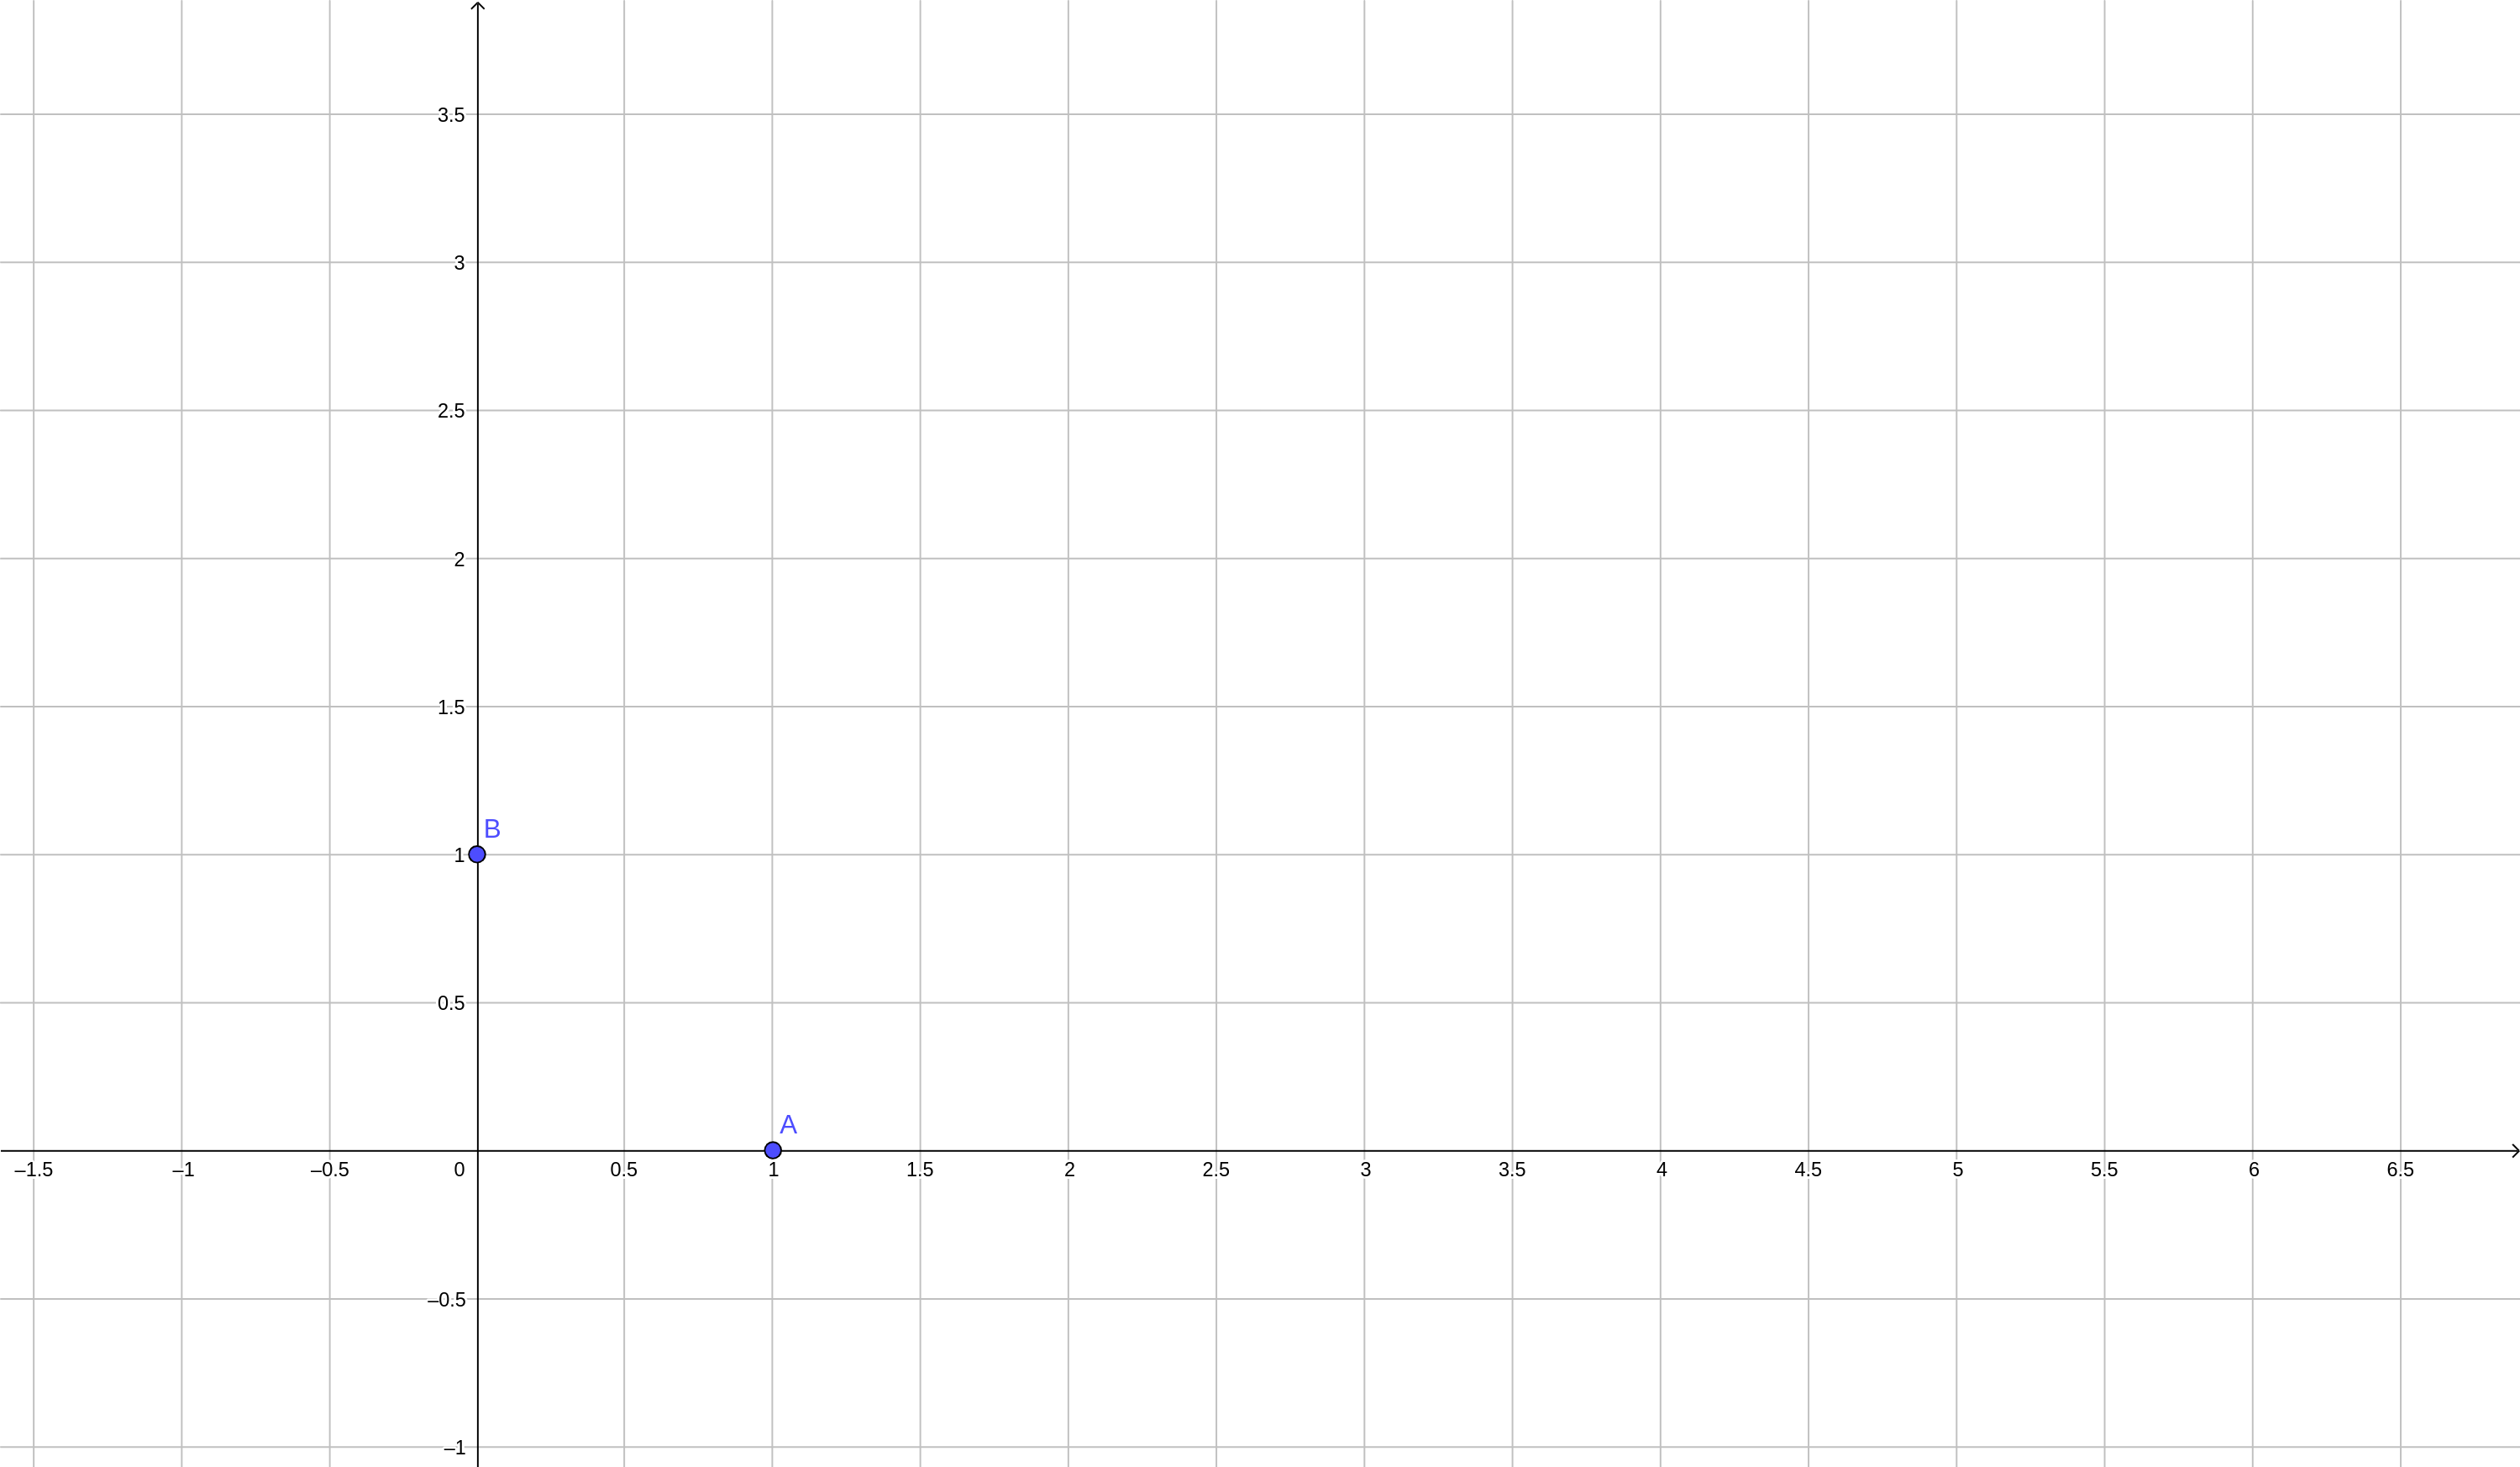
\includegraphics[width=12cm]{grafica1.png}
    \end{figure}

    \item Al reflejar los puntos con respecto al eje $x_1$ se tendrá que quedan en las siguientes posiciones:
    \begin{align*}
        e_1' &= \begin{bmatrix}
            1 \\ 0
        \end{bmatrix} & e_2' &= \begin{bmatrix}
            0 \\ -1
        \end{bmatrix} 
    \end{align*}
    \begin{figure}[h]
        \centering
        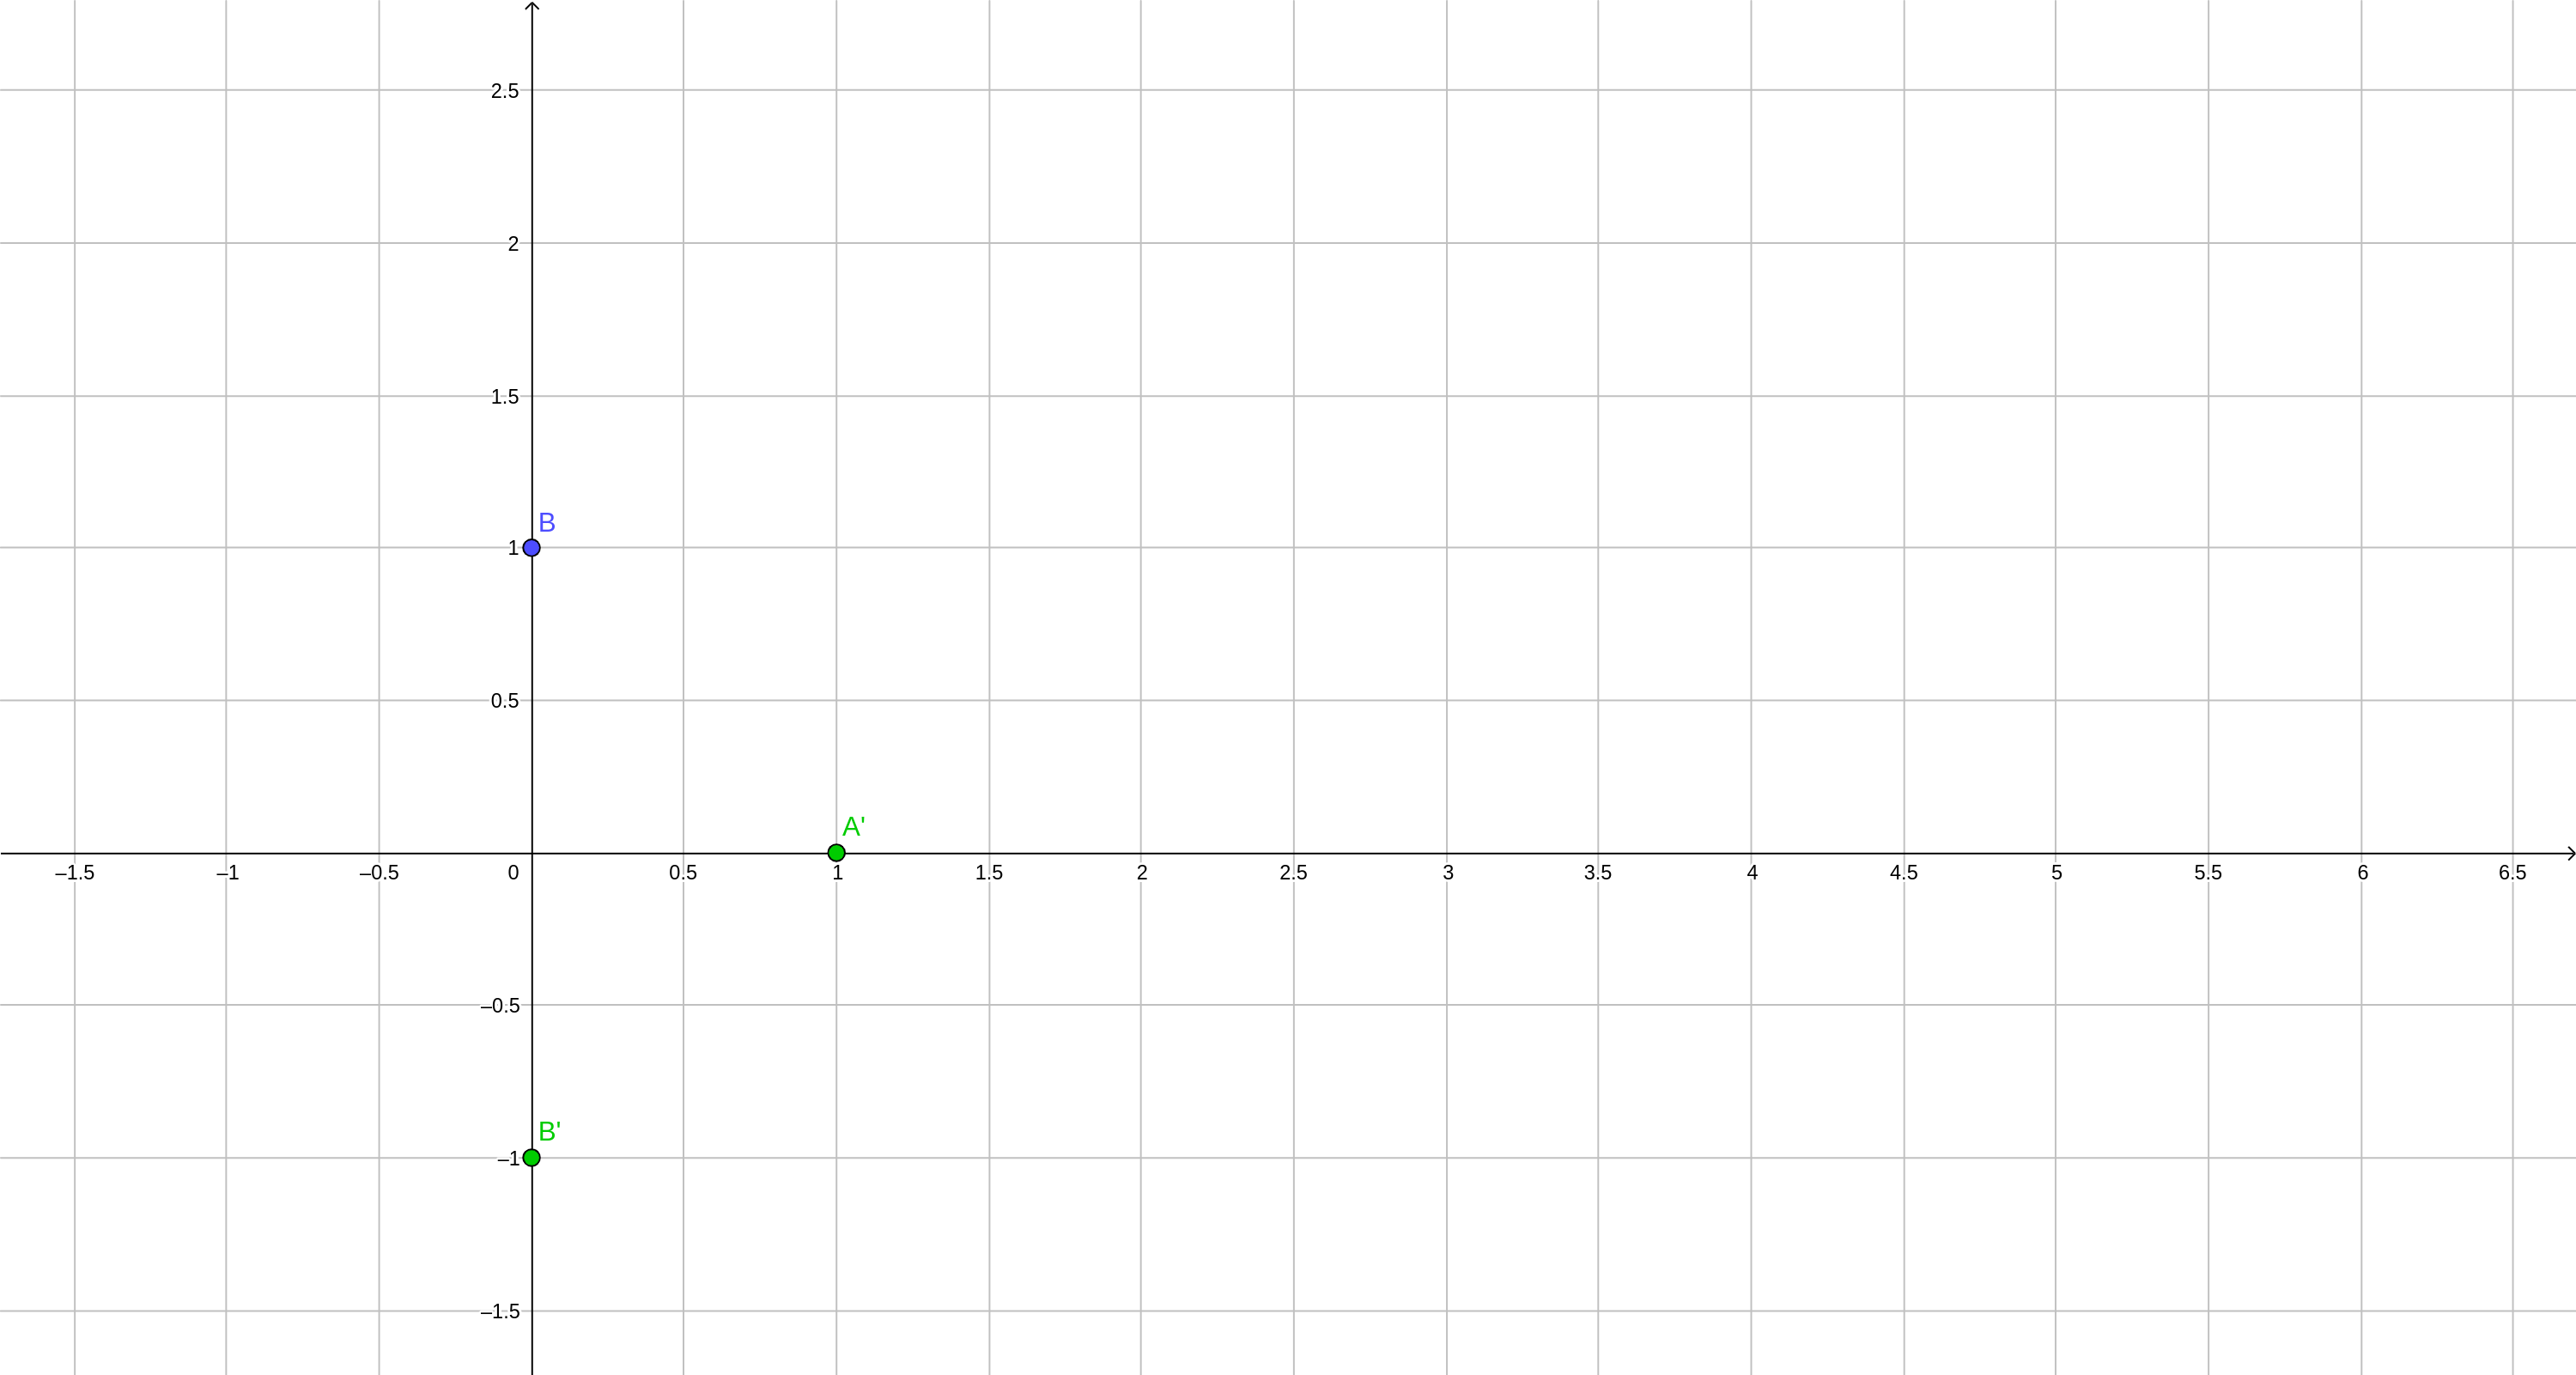
\includegraphics[width=12cm]{grafica2.png}
    \end{figure}

    \item Por último, al reflejar con respecto a la recta $x_2 = x_1$, se tendrán las siguientes transformaciones:
    \begin{align*}
        e_1'' &= \begin{bmatrix}
            0 \\ 1
        \end{bmatrix} & e_2'' &= \begin{bmatrix}
            -1 \\ 0
        \end{bmatrix} 
    \end{align*}
    Si se tiene en cuenta que reflejar sobre $x_2 = x_1$ es igual a intercambiar las coordenadas de las componentes, pues es
    similar al proceso de gráficar una función inversa.
    \begin{figure}[h]
        \centering
        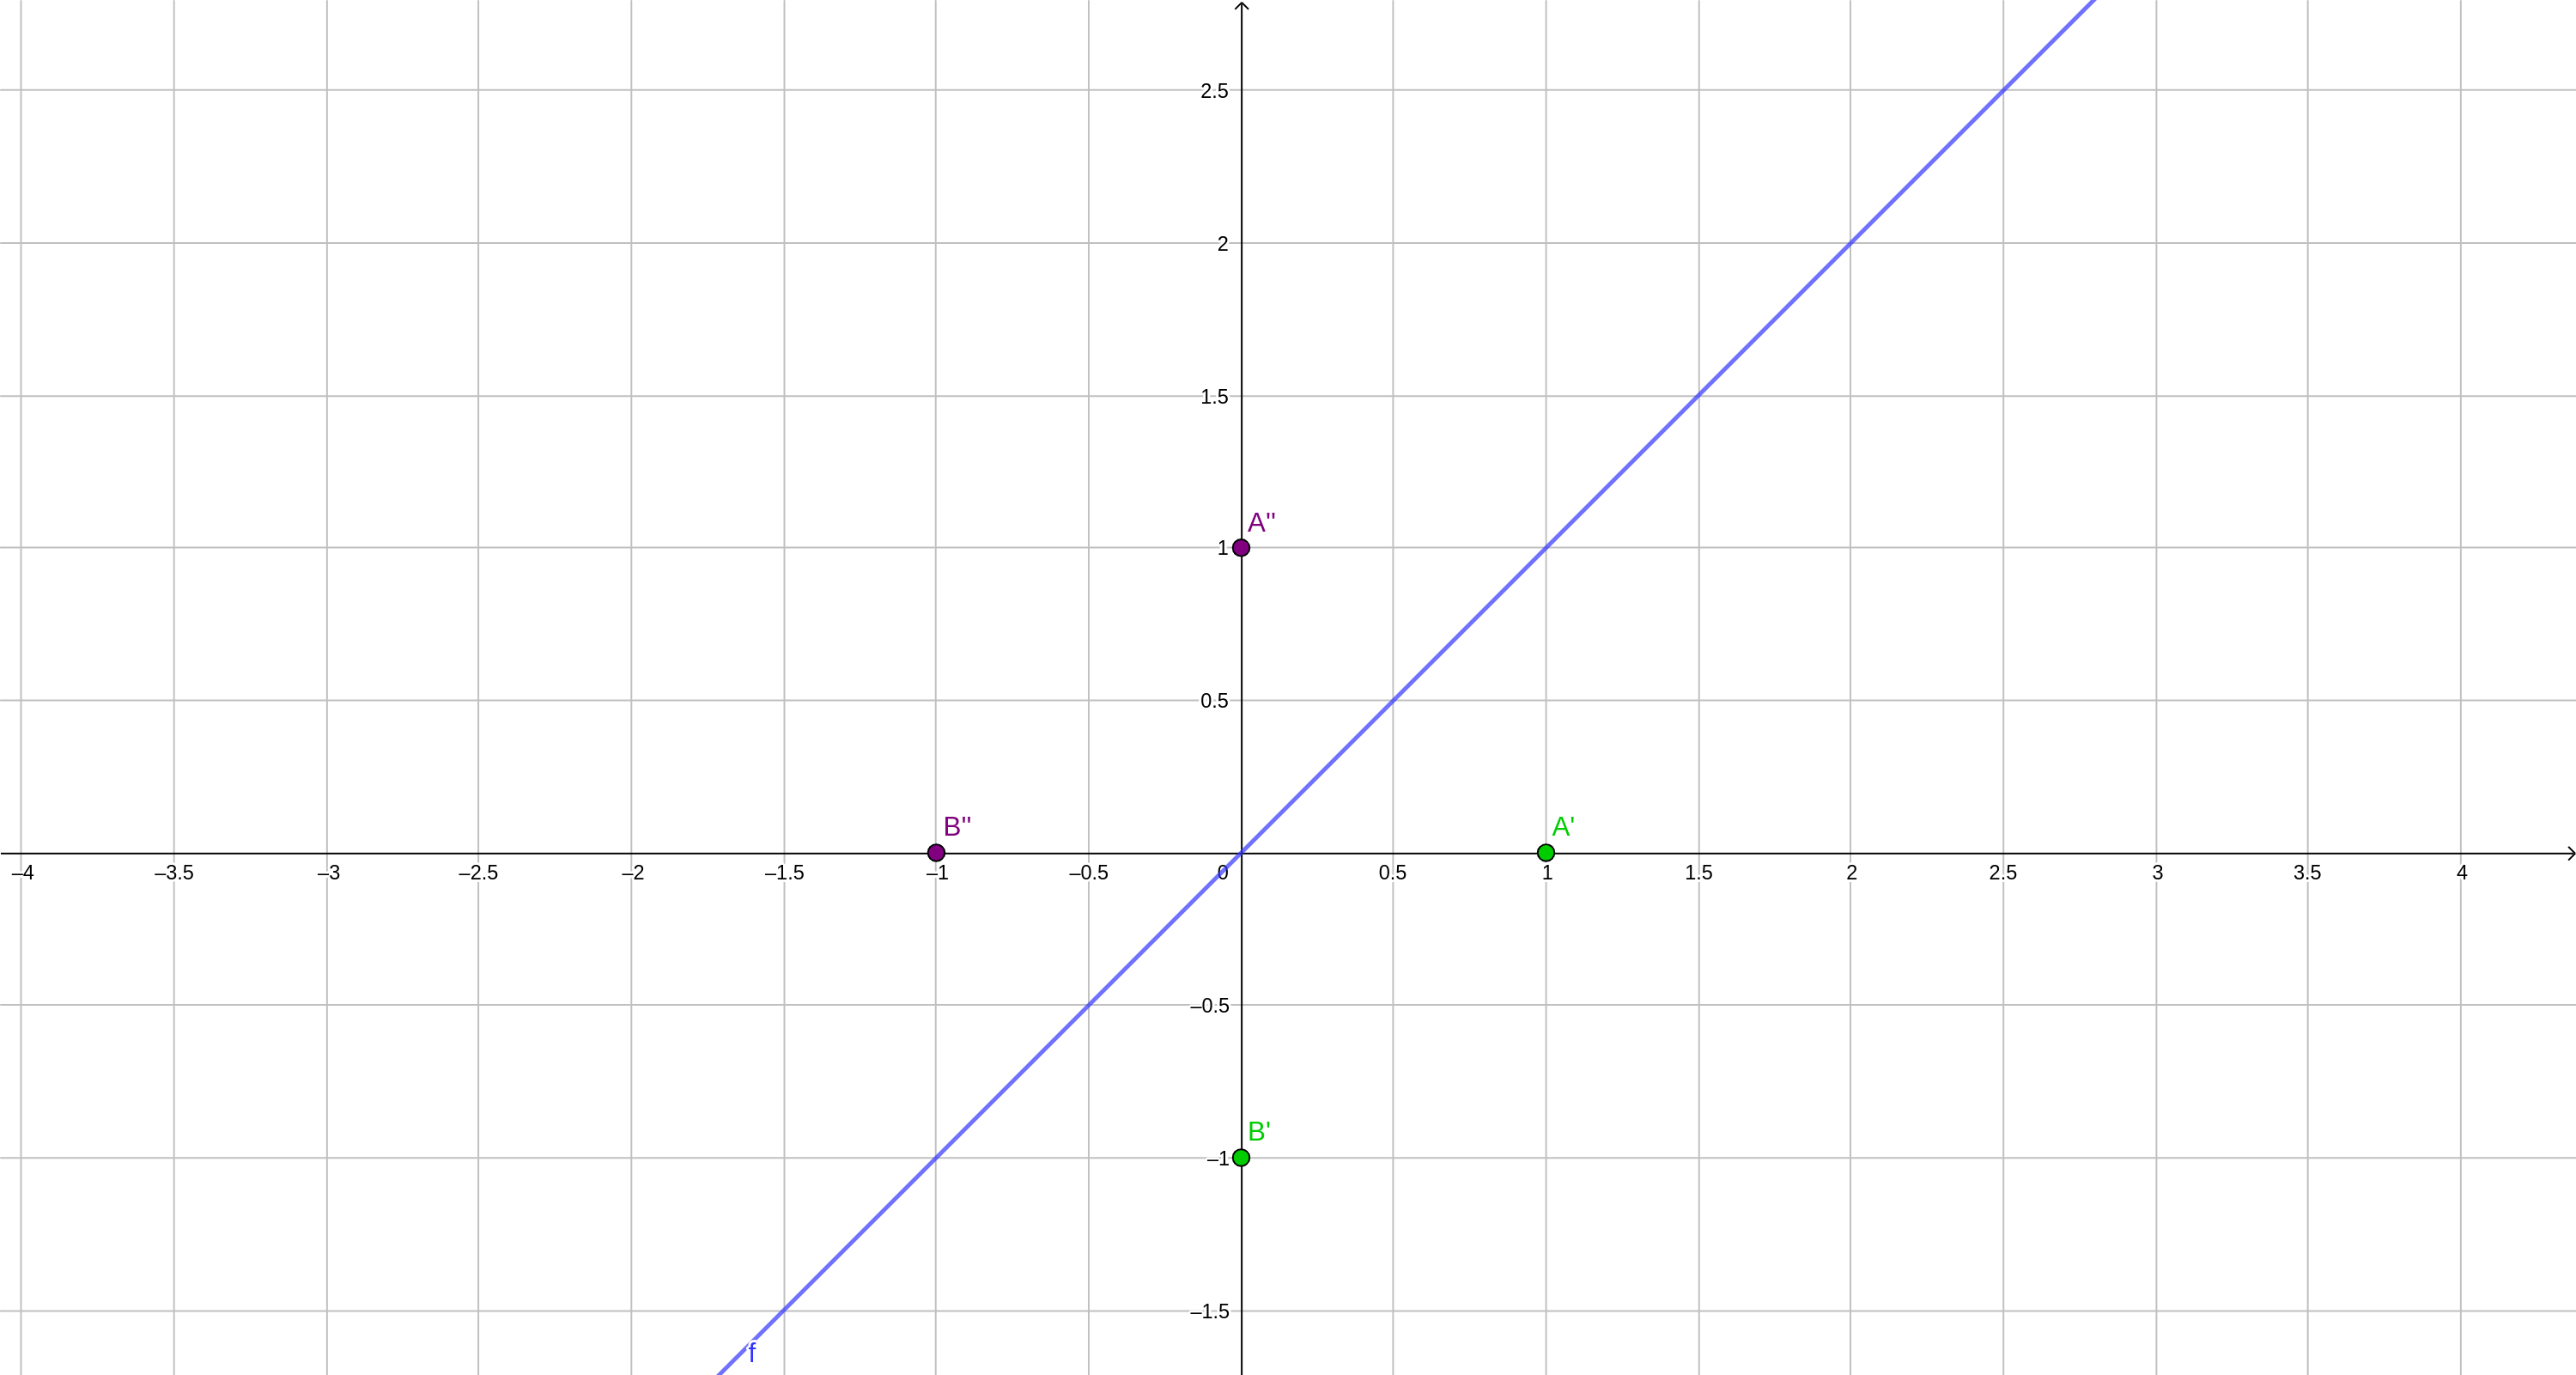
\includegraphics[width=12cm]{grafica3.png}
    \end{figure}
\end{itemize} 
Luego, podremos concluir que los vectores $e_1''$ y $e_2''$ corresponden a las imagenes de $e_1$ y $e_2$ bajo $f$ respectivamente. Por tanto,
la matriz estandar para la transformación $T$ será:
\begin{align*}
    A &= \begin{pmatrix}
        0 & -1\\
        1 & 0\\
    \end{pmatrix}
\end{align*}
\end{questions}
\end{document}